\documentclass[UTF8,12pt,a4paper]{ctexart}

\usepackage{amsmath,amssymb}
\usepackage{graphicx}
\usepackage{geometry}
\usepackage{setspace}
\usepackage{indentfirst}
\usepackage{fancyhdr}
\usepackage{tocloft}
\usepackage{caption}
\usepackage{float}
\usepackage{booktabs}
\usepackage{array}
\usepackage{multirow}
\usepackage{listings}
\usepackage{xcolor}
\usepackage{chngcntr}
\usepackage[hidelinks]{hyperref}

\hypersetup{bookmarksnumbered=true}

\geometry{left=2.5cm,right=2.5cm,top=2.5cm,bottom=2.5cm}
\setlength{\headheight}{14pt}
\graphicspath{{figure/}}
\setlength{\parindent}{2em}
\onehalfspacing

\ctexset{
    section={
        format=\centering\bfseries\zihao{3},
        aftername=\quad,
        beforeskip=1.0ex,
        afterskip=1.0ex
    },
    subsection={
        format=\bfseries\zihao{4},
        beforeskip=0.8ex,
        afterskip=0.8ex
    }
}

\renewcommand{\contentsname}{目录}
\setcounter{tocdepth}{3}
\setcounter{secnumdepth}{3}
\renewcommand{\cftsecfont}{\normalfont\zihao{4}}
\renewcommand{\cftsubsecfont}{\normalfont\zihao{4}}
\renewcommand{\cftsubsubsecfont}{\normalfont\zihao{-4}}
\renewcommand{\cftsecpagefont}{\normalfont\zihao{4}}
\renewcommand{\cftsubsecpagefont}{\normalfont\zihao{4}}
\renewcommand{\cftsubsubsecpagefont}{\normalfont\zihao{-4}}
\setlength{\cftsecindent}{0em}
\setlength{\cftsubsecindent}{2em}
\setlength{\cftsubsubsecindent}{4em}
\setlength{\cftsecnumwidth}{2.2em}
\setlength{\cftsubsecnumwidth}{3.0em}
\setlength{\cftsubsubsecnumwidth}{3.8em}
\renewcommand{\cftsecleader}{\cftdotfill{\cftdotsep}}
\renewcommand{\cftsubsecleader}{\cftdotfill{\cftdotsep}}
\renewcommand{\cftsubsubsecleader}{\cftdotfill{\cftdotsep}}
\setlength{\cftbeforesecskip}{0.1em}
\setlength{\cftbeforesubsecskip}{0.1em}
\setlength{\cftbeforesubsubsecskip}{0.1em}

\counterwithin{figure}{section}
\counterwithin{table}{section}
\renewcommand{\thefigure}{\thesection-\arabic{figure}}
\renewcommand{\thetable}{\thesection-\arabic{table}}

\captionsetup[figure]{labelfont=bf,textfont=normalfont}
\captionsetup[table]{labelfont=bf,textfont=normalfont}
\captionsetup[lstlisting]{labelfont=bf,textfont=normalfont}

\lstset{
    language=Python,
    basicstyle=\ttfamily\small,
    keywordstyle=\color{blue},
    commentstyle=\color{teal!70!black},
    stringstyle=\color{red!70!black},
    numbers=left,
    numberstyle=\tiny\color{gray},
    stepnumber=1,
    numbersep=6pt,
    frame=single,
    breaklines=true,
    showstringspaces=false,
    tabsize=4,
    captionpos=b
}

\pagestyle{fancy}
\fancyhf{}
\fancyhead[C]{\zihao{5}《人工智能》基于 Q-Learning 的强化学习迷宫程序设计报告}
\fancyfoot[C]{\zihao{5}\thepage}
\renewcommand{\headrulewidth}{0.4pt}
\renewcommand{\footrulewidth}{0pt}

\begin{document}

\zihao{4}

% ==================== 封面 ====================
\begin{titlepage}
    \thispagestyle{empty}

    \noindent
    
\includegraphics[width=7.31cm]{school_logo.png}

    \vspace{2.2cm}

    \begin{center}
        {\zihao{-0}\bfseries 《人工智能》\\[0.5em]基于 Q-Learning 的强化学习迷宫程序设计报告}
    \end{center}

    \vspace{3cm}

    \begin{center}
        {\fangsong\zihao{3}
        \begin{tabular}{rl}
            姓\hspace{2em}名: & 余京航 \\[0.5cm]
            班\hspace{2em}级: & 电子2302班 \\[0.5cm]
            学\hspace{2em}号: & 2306020327 \\[0.5cm]
            专\hspace{2em}业: & 电子信息工程 \\[0.5cm]
            学\hspace{2em}院: & 海洋与空间信息学院
        \end{tabular}

        \vspace{3cm}
        2026 年 5 月 2 日
        }
    \end{center}
\end{titlepage}

% ==================== 目录 ====================
\pagenumbering{Roman}
\phantomsection
\noindent\makebox[\textwidth][c]{\bfseries\zihao{3}目录}\par
\vspace{0.3\baselineskip}
\begingroup
\zihao{4}
\makeatletter
\@starttoc{toc}
\makeatother
\endgroup
\newpage

\pagenumbering{arabic}
\setcounter{page}{1}

% ============================================================
\section{实验目的与任务要求}

\subsection{实验背景}
强化学习是机器学习的重要分支，其核心思想是智能体（Agent）通过与环境的交互，根据获得的奖励信号不断调整策略，从而学习到能够最大化累积奖励的行为方式。Q-Learning 是强化学习中最经典的基于价值的算法之一，它通过维护一张状态-动作价值表（Q-table），在不依赖环境模型的情况下实现最优策略的学习。

迷宫导航问题是强化学习教学的经典入门任务。智能体在网格迷宫中从起点出发，需要避开墙壁和陷阱，以最短路径到达终点。该问题直观地展现了"探索-利用"权衡、延迟奖励、信用分配等强化学习核心概念。

\subsection{实验目的}
本实验围绕"基于 Q-Learning 的强化学习迷宫程序设计"展开，主要目标如下：
\begin{enumerate}
    \item 理解强化学习环境中状态空间（State）、动作空间（Action）与奖励机制（Reward）的构建方法。
    \item 手动实现 Q-Learning 算法，掌握 Q-table 的初始化、更新与收敛逻辑。
    \item 利用 Tkinter 实现智能体从随机探索到最优路径的实时可视化展示。
    \item 通过训练日志和评估指标分析智能体的学习过程和策略收敛情况。
\end{enumerate}

\subsection{实验环境}
本实验使用 Python 标准库完成，无需第三方依赖。主要工具如表 \ref{tab:env} 所示。

\begin{table}[H]
\centering
\caption{实验环境与主要工具}
\label{tab:env}
\begin{tabular}{>{\centering\arraybackslash}p{3.5cm}>{\centering\arraybackslash}p{8.5cm}}
\toprule
项目 & 内容 \\
\midrule
编程语言 & Python 3.13 \\
开发框架 & 仅 Python 标准库 \\
可视化工具 & Tkinter（可选） \\
训练记录格式 & JSON \\
随机种子 & 42（可配置） \\
\bottomrule
\end{tabular}
\end{table}

% ============================================================
\section{Q-Learning 算法原理}

\subsection{马尔可夫决策过程}
强化学习问题通常建模为马尔可夫决策过程（MDP），由五元组 $(S, A, P, R, \gamma)$ 描述。在迷宫问题中：
\begin{itemize}
    \item 状态空间 $S$：智能体在网格中的坐标 $(x, y)$，共 $10 \times 10 = 100$ 个可能位置。
    \item 动作空间 $A$：上、下、左、右四个离散动作，编码为 $\{0, 1, 2, 3\}$。
    \item 状态转移概率 $P$：由环境确定，尝试越界或撞墙时停留在原地。
    \item 奖励函数 $R$：终点 +1，撞墙/陷阱 -1，每步 -0.01。
    \item 折扣因子 $\gamma$：取 0.95，平衡即时奖励与长期回报。
\end{itemize}

\subsection{Q-Learning 更新公式}
Q-Learning 是一种 off-policy 的时序差分算法，其核心更新公式为：
\begin{equation}
Q(s, a) \leftarrow Q(s, a) + \alpha \left[ r + \gamma \max_{a'} Q(s', a') - Q(s, a) \right]
\end{equation}
其中，$Q(s, a)$ 表示在状态 $s$ 下执行动作 $a$ 的期望累积奖励估计值，$\alpha$ 为学习率。更新过程通过当前奖励 $r$ 和下一状态的最优 Q 值来修正当前估计，使 Q 值逐步逼近真实最优价值函数 $Q^*(s, a)$。

\subsection{Epsilon-Greedy 探索策略}
为了平衡探索与利用，智能体采用 epsilon-greedy 策略选择动作：
\begin{equation}
\pi(a|s) = \begin{cases}
\text{随机动作}, & \text{概率 } \epsilon \\
\arg\max_a Q(s, a), & \text{概率 } 1 - \epsilon
\end{cases}
\end{equation}
训练开始时 $\epsilon = 1.0$，智能体以纯随机方式探索；每回合结束后 $\epsilon$ 乘以衰减系数 $0.995$，逐步降低到最小值 $0.08$，使智能体从探索为主过渡到利用为主。

\subsection{奖励塑造}
奖励函数的设计直接影响学习效率和质量。本实验的奖励设置如下：
\begin{itemize}
    \item \textbf{到达终点（+1）}：正反馈，引导智能体以终点为目标。
    \item \textbf{撞墙或越界（-1）}：强负反馈，快速压低无效动作的 Q 值。
    \item \textbf{掉入陷阱（-1）}：与撞墙同等的负反馈，同时终止回合。
    \item \textbf{每步移动（-0.01）}：微小负奖励，鼓励寻找最短路径。
\end{itemize}
注意，撞墙并不终止回合——智能体停留在原地并可在下一步选择其他动作。这种设计在包含动态障碍的较大地图上有助于提高学习效率。

% ============================================================
\section{软件架构设计}

本设计采用模块化结构，将逻辑与显示分离，分为三个核心模块，其关系如图 \ref{fig:architecture} 所示。

\begin{figure}[H]
    \centering
    \begin{minipage}{0.9\textwidth}
    \centering
    \begin{tabular}{|c|c|}
    \hline
    \textbf{模块} & \textbf{职责} \\
    \hline
    main.py & 训练循环、可视化、记录回放、策略评估 \\
    \hline
    maze\_env.py & Gym 风格迷宫环境、状态转移与奖励计算 \\
    \hline
    rl\_brain.py & Q-table 维护、动作选择与 Q 值更新 \\
    \hline
    \end{tabular}
    \caption{模块架构}
    \label{fig:architecture}
    \end{minipage}
\end{figure}

\subsection{迷宫环境模块（maze\_env.py）}
环境模块采用 Gym 风格的接口设计，提供 \texttt{reset()} 和 \texttt{step()} 两个核心方法。\texttt{reset()} 重置智能体到起点并刷新动态障碍，\texttt{step(action)} 执行动作并返回下一状态、奖励、结束标志和信息字典。环境支持静态墙壁、固定陷阱和每回合随机刷新的动态墙壁。

\subsection{强化学习大脑模块（rl\_brain.py）}
智能体模块维护一张以状态为键、动作价值列表为值的 Q-table。当遇到未访问过的状态时，自动初始化该状态的所有动作 Q 值为 0。\texttt{choose\_action()} 实现 epsilon-greedy 策略，\texttt{learn()} 实现 Q-Learning 更新公式，\texttt{decay\_epsilon()} 每回合衰减探索率。

\subsection{主循环模块（main.py）}
主模块负责将环境与智能体串联，具体包括：
\begin{itemize}
    \item \texttt{train\_agent()}：多回合训练循环，记录每回合路径、奖励和成功率。
    \item \texttt{evaluate\_policy()}：训练后以纯贪心策略评估智能体性能。
    \item \texttt{run\_greedy\_episode()}：可视化展示训练后的最优路径。
    \item \texttt{replay\_training\_history()}：回放训练过程中的路径演化。
\end{itemize}

% ============================================================
\section{训练方法与评估设置}

\subsection{训练流程}
每个训练回合的执行流程如下：
\begin{enumerate}
    \item \texttt{env.reset()} 重置环境，智能体回到起点 $(0, 0)$，动态墙壁随机刷新。
    \item 循环执行以下步骤，直到到达终点、掉入陷阱或步数超过上限：
    \begin{itemize}
        \item \texttt{agent.choose\_action(state)} 根据 epsilon-greedy 策略选择动作。
        \item \texttt{env.step(action)} 执行动作，获得下一状态和奖励。
        \item \texttt{agent.learn()} 根据 Q-Learning 公式更新 Q-table。
    \end{itemize}
    \item 回合结束后调用 \texttt{agent.decay\_epsilon()} 衰减探索率。
    \item 每 20 回合输出一次训练日志（平均奖励、成功率、epsilon、Q 表大小）。
\end{enumerate}

\subsection{训练参数}
训练参数设置如表 \ref{tab:train-params} 所示。

\begin{table}[H]
\centering
\caption{训练参数设置}
\label{tab:train-params}
\begin{tabular}{>{\centering\arraybackslash}p{4cm}>{\centering\arraybackslash}p{4cm}>{\centering\arraybackslash}p{4cm}}
\toprule
参数 & 取值 & 说明 \\
\midrule
回合数 & 300 & 训练总轮次 \\
最大步数 & 220 & 每回合步数上限 \\
学习率 $\alpha$ & 0.1 & Q 值更新步长 \\
折扣因子 $\gamma$ & 0.95 & 长期回报权重 \\
初始 $\epsilon$ & 1.0 & 初始探索率 \\
$\epsilon$ 最小值 & 0.08 & 探索率下限 \\
$\epsilon$ 衰减率 & 0.995 & 每回合衰减系数 \\
随机种子 & 42 & 结果可复现 \\
\bottomrule
\end{tabular}
\end{table}

\subsection{评估方法}
训练完成后进行两个维度的评估：
\begin{enumerate}
    \item \textbf{贪心策略评估}：关闭探索，使用纯贪心策略连续运行 40 回合，统计成功率和平均步数。
    \item \textbf{演示运行}：以贪心策略运行一回合并可视化展示，观察路径质量。
\end{enumerate}

% ============================================================
\section{实验结果与分析}

\subsection{训练日志分析}
训练过程中每 20 回合记录的日志数据如图 \ref{fig:train-log} 和图 \ref{fig:train-log2} 所示。

\begin{figure}[H]
    \centering
    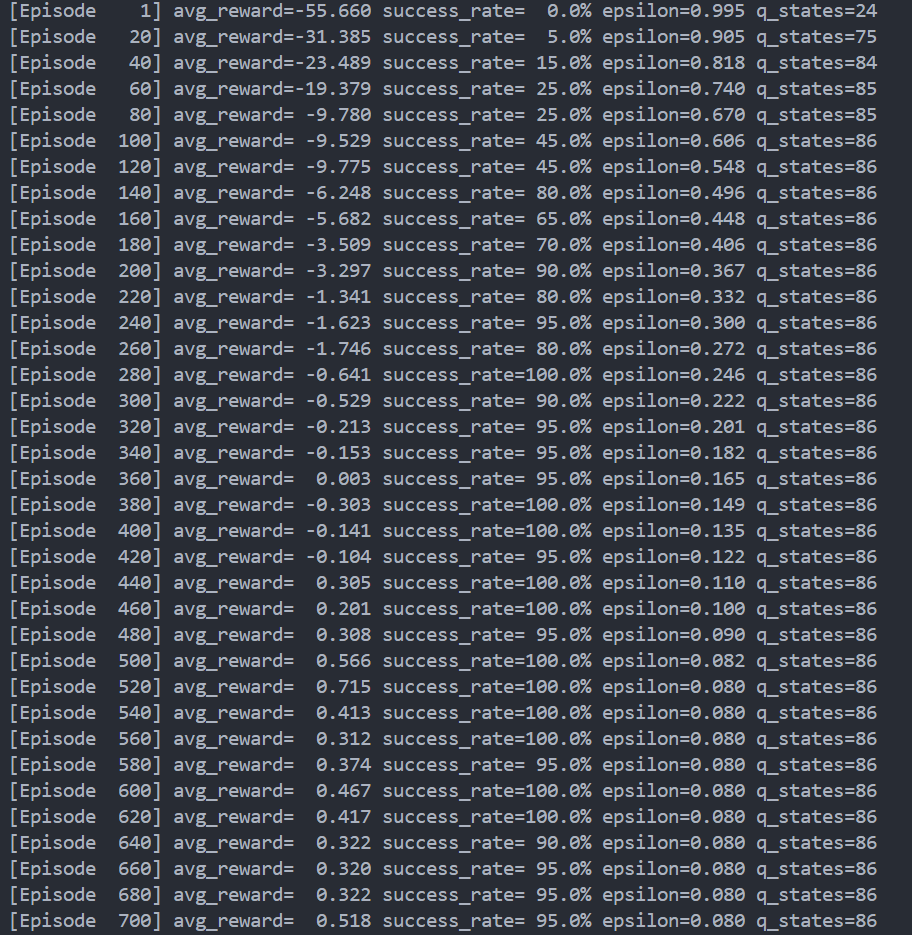
\includegraphics[width=1.0\textwidth]{训练日志图.png}
    \caption{训练日志（前半段）}
    \label{fig:train-log}
\end{figure}

\begin{figure}[H]
    \centering
    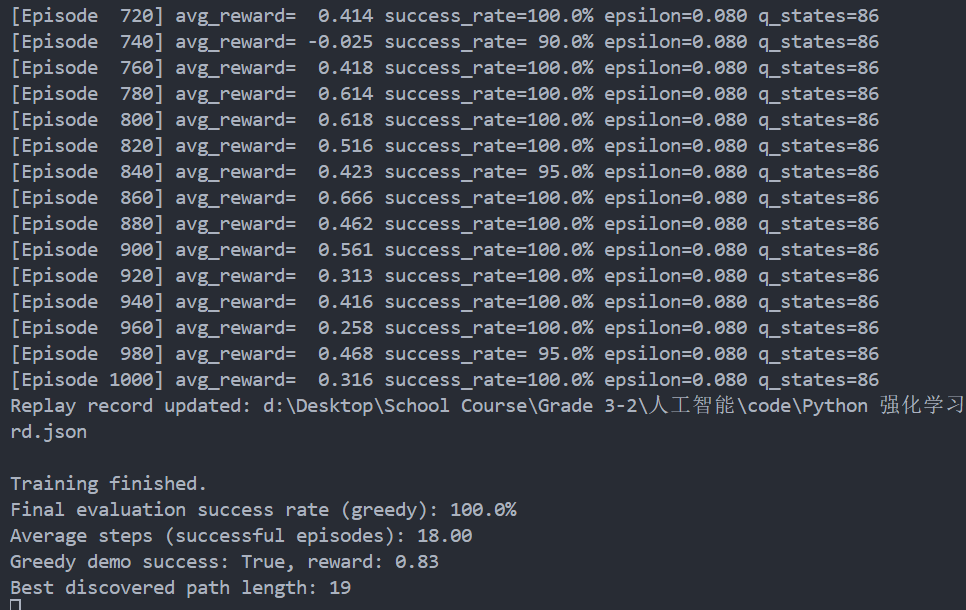
\includegraphics[width=1.0\textwidth]{训练日志图续.png}
    \caption{训练日志（后半段）}
    \label{fig:train-log2}
\end{figure}

从日志数据可以看出，训练过程呈现出以下规律：
\begin{itemize}
    \item \textbf{平均奖励}：从第 1 回合的 -55.66 持续上升到第 300 回合的 -0.53，说明智能体逐步学会了以更短的路径到达终点。
    \item \textbf{成功率}：从初始的 0\% 逐步提高到第 280 回合的 100\%，表明智能体在后期几乎每回合都能成功到达终点。
    \item \textbf{Epsilon 衰减}：从 1.0 逐步衰减到 0.222，体现了从随机探索到确定性利用的过渡过程。
    \item \textbf{Q 表规模}：Q 表在约 100 回合后稳定在 86 个状态，说明智能体已基本探索完迷宫中的所有可达位置。
\end{itemize}

\subsection{训练过程可视化}
图 \ref{fig:train-compare} 对比展示了训练早期（第 8 回合）和中期（第 46 回合）智能体的探索情况。

\begin{figure}[H]
    \centering
    \begin{minipage}{0.48\textwidth}
        \centering
        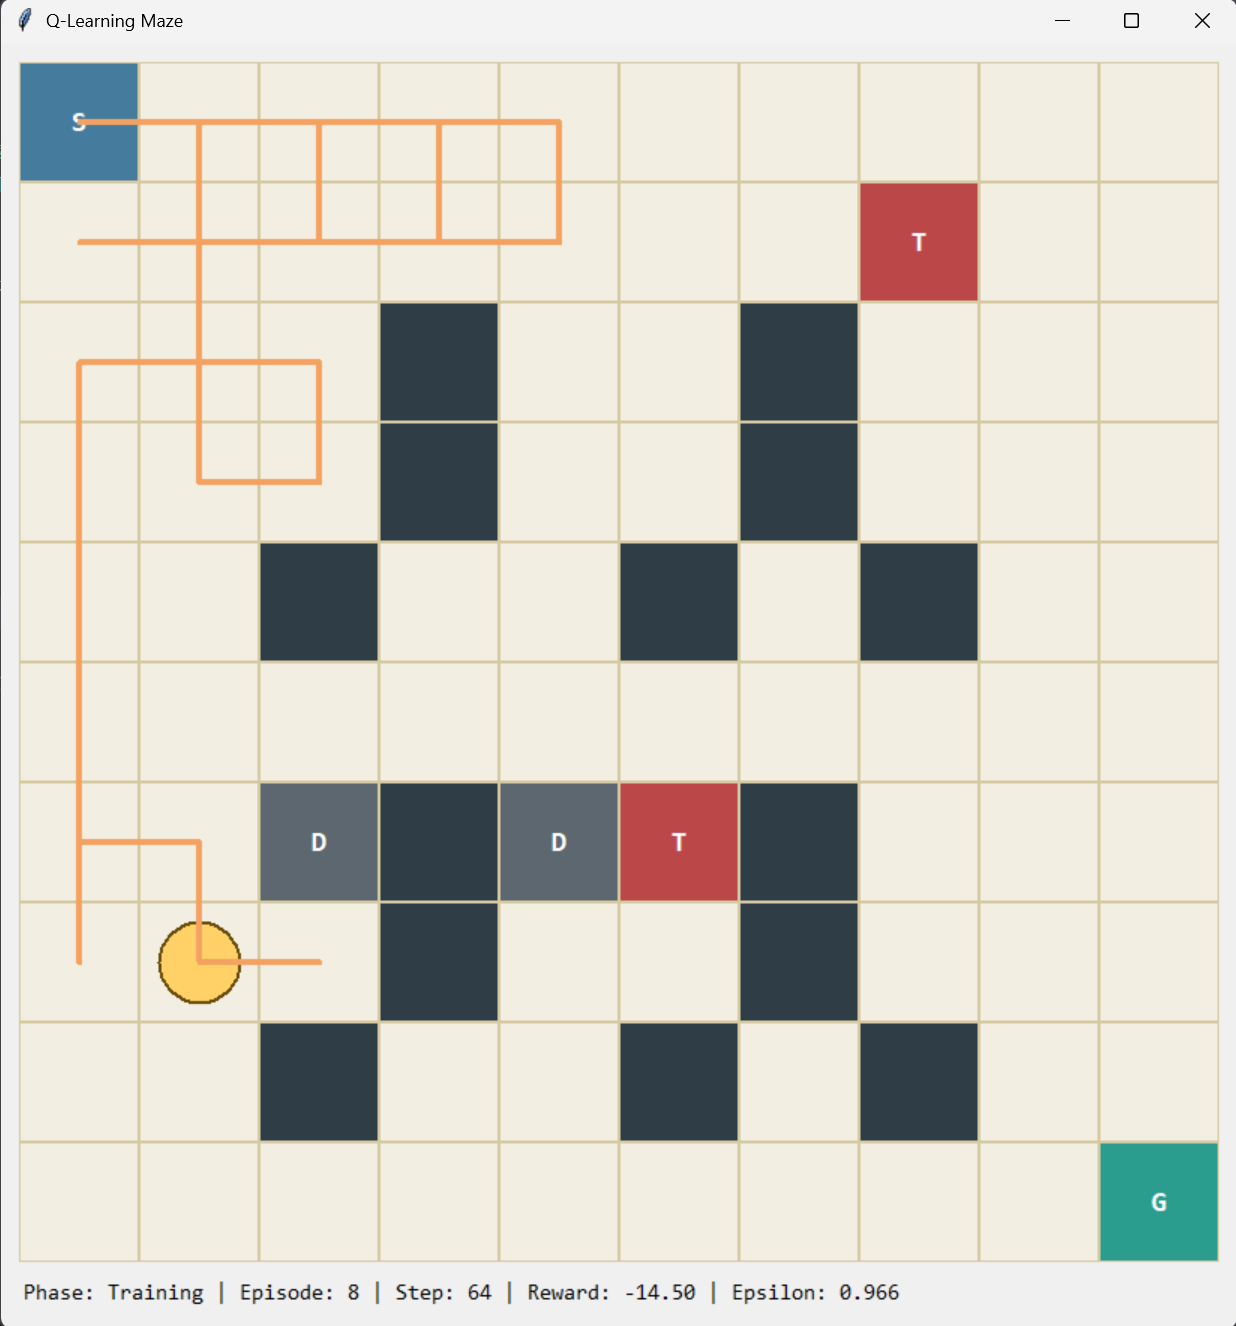
\includegraphics[width=\textwidth]{训练过程图（第8轮）.png}
        \caption{第 8 回合——早期随机探索}
        \label{fig:ep8}
    \end{minipage}
    \hfill
    \begin{minipage}{0.48\textwidth}
        \centering
        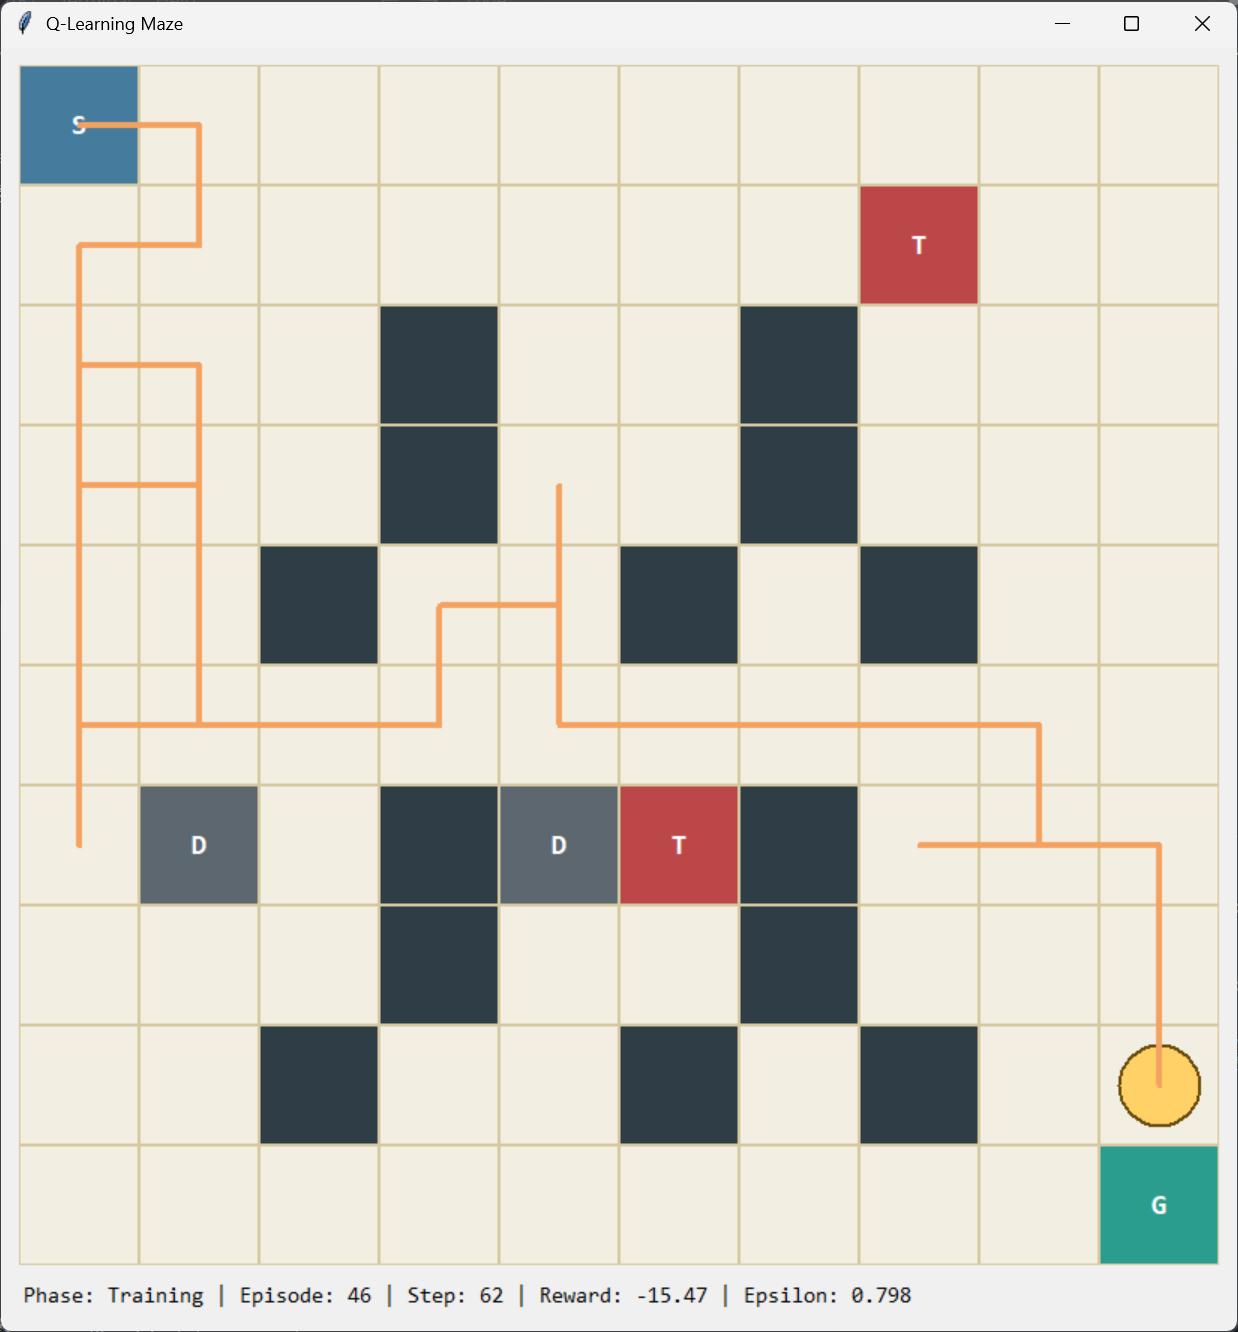
\includegraphics[width=\textwidth]{训练过程图（第46轮）.png}
        \caption{第 46 回合——策略逐渐成形}
        \label{fig:ep46}
    \end{minipage}
    \caption{训练过程对比}
    \label{fig:train-compare}
\end{figure}

早期训练中智能体尚未形成有效策略，路径杂乱无章，经常撞墙或掉入陷阱。这是因为 $\epsilon$ 值仍然较高（第 8 回合约 0.96），随机探索占主导地位。

到第 46 回合时，智能体已经能够找到终点，但路径仍然包含较多不必要的绕行。此时 $\epsilon$ 约 0.79，仍有相当的探索概率，但 Q 表已经积累了一定经验，方向性明显改善。

\subsection{最终策略评估}
训练结束后，以纯贪心策略（$\epsilon = 0$）评估智能体性能，40 轮评估结果如表 \ref{tab:eval} 所示。

\begin{table}[H]
\centering
\caption{最终策略评估结果}
\label{tab:eval}
\begin{tabular}{>{\centering\arraybackslash}p{5cm}>{\centering\arraybackslash}p{5cm}}
\toprule
指标 & 结果 \\
\midrule
贪心评估成功率 & 100.0\% \\
平均步数（成功回合） & 18.00 步 \\
演示运行成功 & 是 \\
演示运行奖励 & 0.83 \\
最优路径长度 & 19 步（含起点） \\
\bottomrule
\end{tabular}
\end{table}

100\% 的成功率和 18 步的平均步数表明，经过 300 回合训练，智能体已经学到了稳定的最优策略。图 \ref{fig:final} 展示了训练后的最优路径。

\begin{figure}[H]
    \centering
    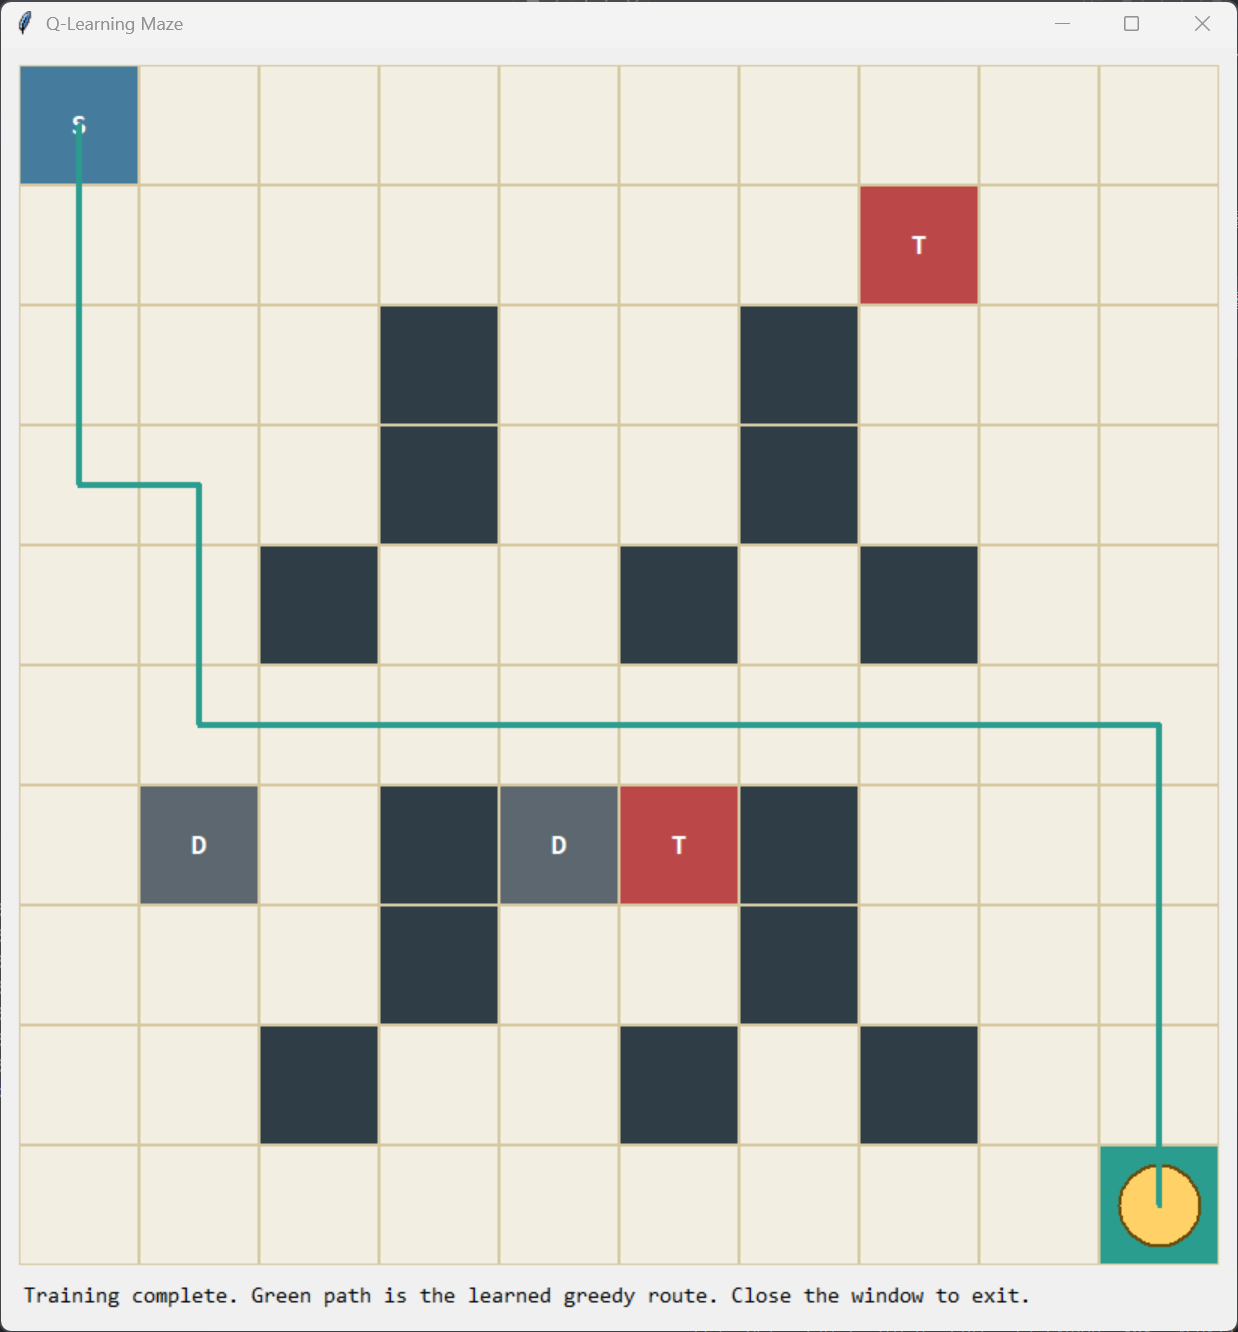
\includegraphics[width=0.6\textwidth]{最终成功图回溯.png}
    \caption{训练后的最优路径回溯}
    \label{fig:final}
\end{figure}

% ============================================================
\section{关键代码说明}

\subsection{环境模块核心逻辑}
环境模块的核心是 \texttt{step()} 方法，它根据动作计算下一位置并确定奖励：

\begin{lstlisting}[caption={迷宫环境 step 方法核心逻辑}]
def step(self, action):
    self.steps_taken += 1
    dx, dy = ACTION_DELTAS[action]
    nx, ny = self.state[0] + dx, self.state[1] + dy
    next_state = (nx, ny)

    reward = self.step_penalty  # -0.01

    if (not self._in_bounds(next_state)) or (next_state in self.walls):
        reward = self.wall_penalty  # -1，不终止回合
    elif next_state in self.traps:
        self.state = next_state
        reward = self.trap_penalty
        self.done = True
    elif next_state == self.goal:
        self.state = next_state
        reward = self.goal_reward  # +1
        self.done = True
    else:
        self.state = next_state

    return self.state, reward, self.done, info
\end{lstlisting}

注意撞墙处理与其他障碍的区别：撞墙时智能体不移动、不终止回合，仅获得负奖励，以便在动态障碍环境中继续学习。

\subsection{Q-Learning 更新实现}
Q 表更新是算法的核心，实现如下：

\begin{lstlisting}[caption={Q-Learning 更新逻辑}]
def learn(self, state, action, reward, next_state, done):
    current_values = self.q_table[state]
    next_values = self.q_table[next_state]

    predict = current_values[action]
    target = reward if done else reward + self.gamma * max(next_values)

    current_values[action] += self.learning_rate * (target - predict)
\end{lstlisting}

当 \texttt{done=True} 时，目标值仅包含即时奖励（终态无后续 Q 值）；否则使用 Bellman 方程计算含折扣的未来回报。

\subsection{训练循环与可视化}
训练循环将环境交互、Q 值更新和可视化渲染串接：

\begin{lstlisting}[caption={训练循环主框架}]
for episode in range(1, episodes + 1):
    state = env.reset()
    episode_reward = 0.0
    path = [state]

    for step in range(1, max_steps + 1):
        action = agent.choose_action(state, training=True)
        next_state, reward, done, _ = env.step(action)
        agent.learn(state, action, reward, next_state, done)

        state = next_state
        episode_reward += reward
        path.append(state)

        if done:
            break

    success = state == env.goal
    agent.decay_epsilon()
\end{lstlisting}

% ============================================================
\section{问题分析与改进方向}

\subsection{存在问题}
实验结果表明，当前智能体已能成功学习到迷宫中的最优路径，但仍存在以下可改进之处：
\begin{enumerate}
    \item \textbf{Q 表泛化能力有限}：表格型 Q-Learning 需要逐个状态独立学习，对于更大规模的迷宫，状态空间爆炸会导致 Q 表无法维护。
    \item \textbf{动态障碍适应性不足}：每回合重新采样的动态墙壁可能导致智能体在少数回合中遇到未见过的障碍布局，从而失败。
    \item \textbf{训练后期探索不足}：当 $\epsilon$ 衰减到较低水平后，智能体可能无法适应环境变化。
    \item \textbf{无经验回放}：当前实现每条经验只使用一次即丢弃，样本效率较低。
\end{enumerate}

\subsection{改进方向}
后续可从以下方向继续优化：
\begin{enumerate}
    \item 使用函数逼近方法（如 DQN）替代表格型 Q-Learning，以处理更大规模的状态空间。
    \item 引入经验回放机制，提高样本利用率，降低训练所需回合数。
    \item 增加 $\epsilon$ 的重置或循环机制，使智能体在后期仍保持适度的探索能力。
    \item 扩展为更复杂的迷宫布局（如随机生成地图），测试算法的泛化性能。
    \item 对比不同奖励设计（如撞墙终止 vs. 不终止）对学习效果的影响。
\end{enumerate}

% ============================================================
\section{实验总结}

本实验完成了一个基于 Q-Learning 的强化学习迷宫程序设计与实现。实验首先构建了 Gym 风格的 10×10 网格迷宫环境，包含静态墙壁、固定陷阱和每回合随机刷新的动态墙壁；随后实现了表格型 Q-Learning 智能体，通过 epsilon-greedy 策略平衡探索与利用；最后通过 Tkinter 可视化展示了智能体从随机探索到最优路径的完整学习过程。

从实验结果看，经过 300 回合训练，智能体的成功率达到 100\%，平均步数为 18 步，贪心策略评估准确率为 100\%。训练日志显示平均奖励从 -55.66 持续上升到 -0.53，Q 表在约 100 回合后稳定在 86 个状态。实验结果表明，Q-Learning 算法能够有效地在网格迷宫环境中学习到最优导航策略。

本实验完整覆盖了强化学习环境建模、Q-Learning 算法实现、训练与评估流程以及可视化展示，加深了对强化学习中"探索-利用"权衡、时序差分学习和奖励塑造等核心概念的理解。

\end{document}
